\section{Parts choice} \label{sec:parts_choice}
During the development phase of the project, some hardware components needed to be chosen in order for us to be able to actually develop a prototype system.
With components ranging from a full computing platform to a simple electrical connection board, we will briefly introduce the necessary hardware as well as provide an explanation about the logic utilized during the decision period.

% Parts choice
% `- Motor & Encoder
% `- DFR0592
% `- Raspberry Pi
% `- netHAT 52-RTE
% `- screw terminal add-on

\subsection{Raspberry Pi 4} \label{subsec:rpi4}
The Raspberry Pi 4 is a single board computer (SBC) and comes equipped with the Broadcom's BCM2711, a quad-core Cortex-A72 64-bit ARM processor clocked at 1.5 GHz \cite{technology:rpi4-specs}.
At the time of writing, versions were available with 2 GB, 4 GB and 8 GB of LPDDR4 SD-RAM \footnote{Low-Power Double Data Rate Synchronous Dynamic Random-Access Memory} clocked at 3200 MHz.

This version of the Raspberry Pi series is the first to be equipped with a true-Gigabit Ethernet controller connected to the PCIe bus, while earlier versions used a USB attached one, meaning latency and throughput were not as good and especially less constant.

As our designed slave device is intended to be used in headless mode, meaning no monitor output and no keyboard nor mouse will be used, we picked the version with 2GB of RAM.
As no graphical interface needs to be created, memory usage will be very reduced and, as such, 2GB are plenty of memory for our needs.

The Raspberry Pi 4 incorporates a micro-SD card slot to be used as an embedded hard disk, so we have also included a small 16GB micro-SD card to serve as such.
Linux is a very small operating system and a fresh install of Raspberry Pi OS Lite occupies about 1.4GB, meaning the 16GB of space are more than sufficient for our needs.

% Conclusion
During the development phase we have considered the Raspberry Pi 4 to be the most appropriate solution for the project's slave computing platform.
Its features and characteristics seemed to fit the requirements well, so we locked our choice for this equipment.

\subsection{Motor \& encoder}
% `- DC motor
% `- Encoder
% `- Why not standard servo motor + drive
In order to provide our system with the physical connection with the world we aim for, we have chosen a small 6V brushed DC motor with an embedded 30:1 gearbox \cite{product:pololu-micrometal-gearmotor}.
This motor provides an extended shaft on the back of the motor so that a magnetic encoder kit can be attached to it.

Pololu \cite{brand:pololu}, which is the maker of our chosen motor, separately provides the magnetic quadrature encoder kit, compatible with such motor, with a resolution of 12 pulses per revolution (PPR) in quadrature mode.
A preview picture of the motor + encoder kit can be seen in \autoref{fig:encoder_motor}.
The encoder provides quadrature signals A and B at the same voltage as its power supply.
It is rated to be powered between 2.7V and 18V, allowing it to used for a wide variety of applications.

\begin{figure}[htp]
	\centering
	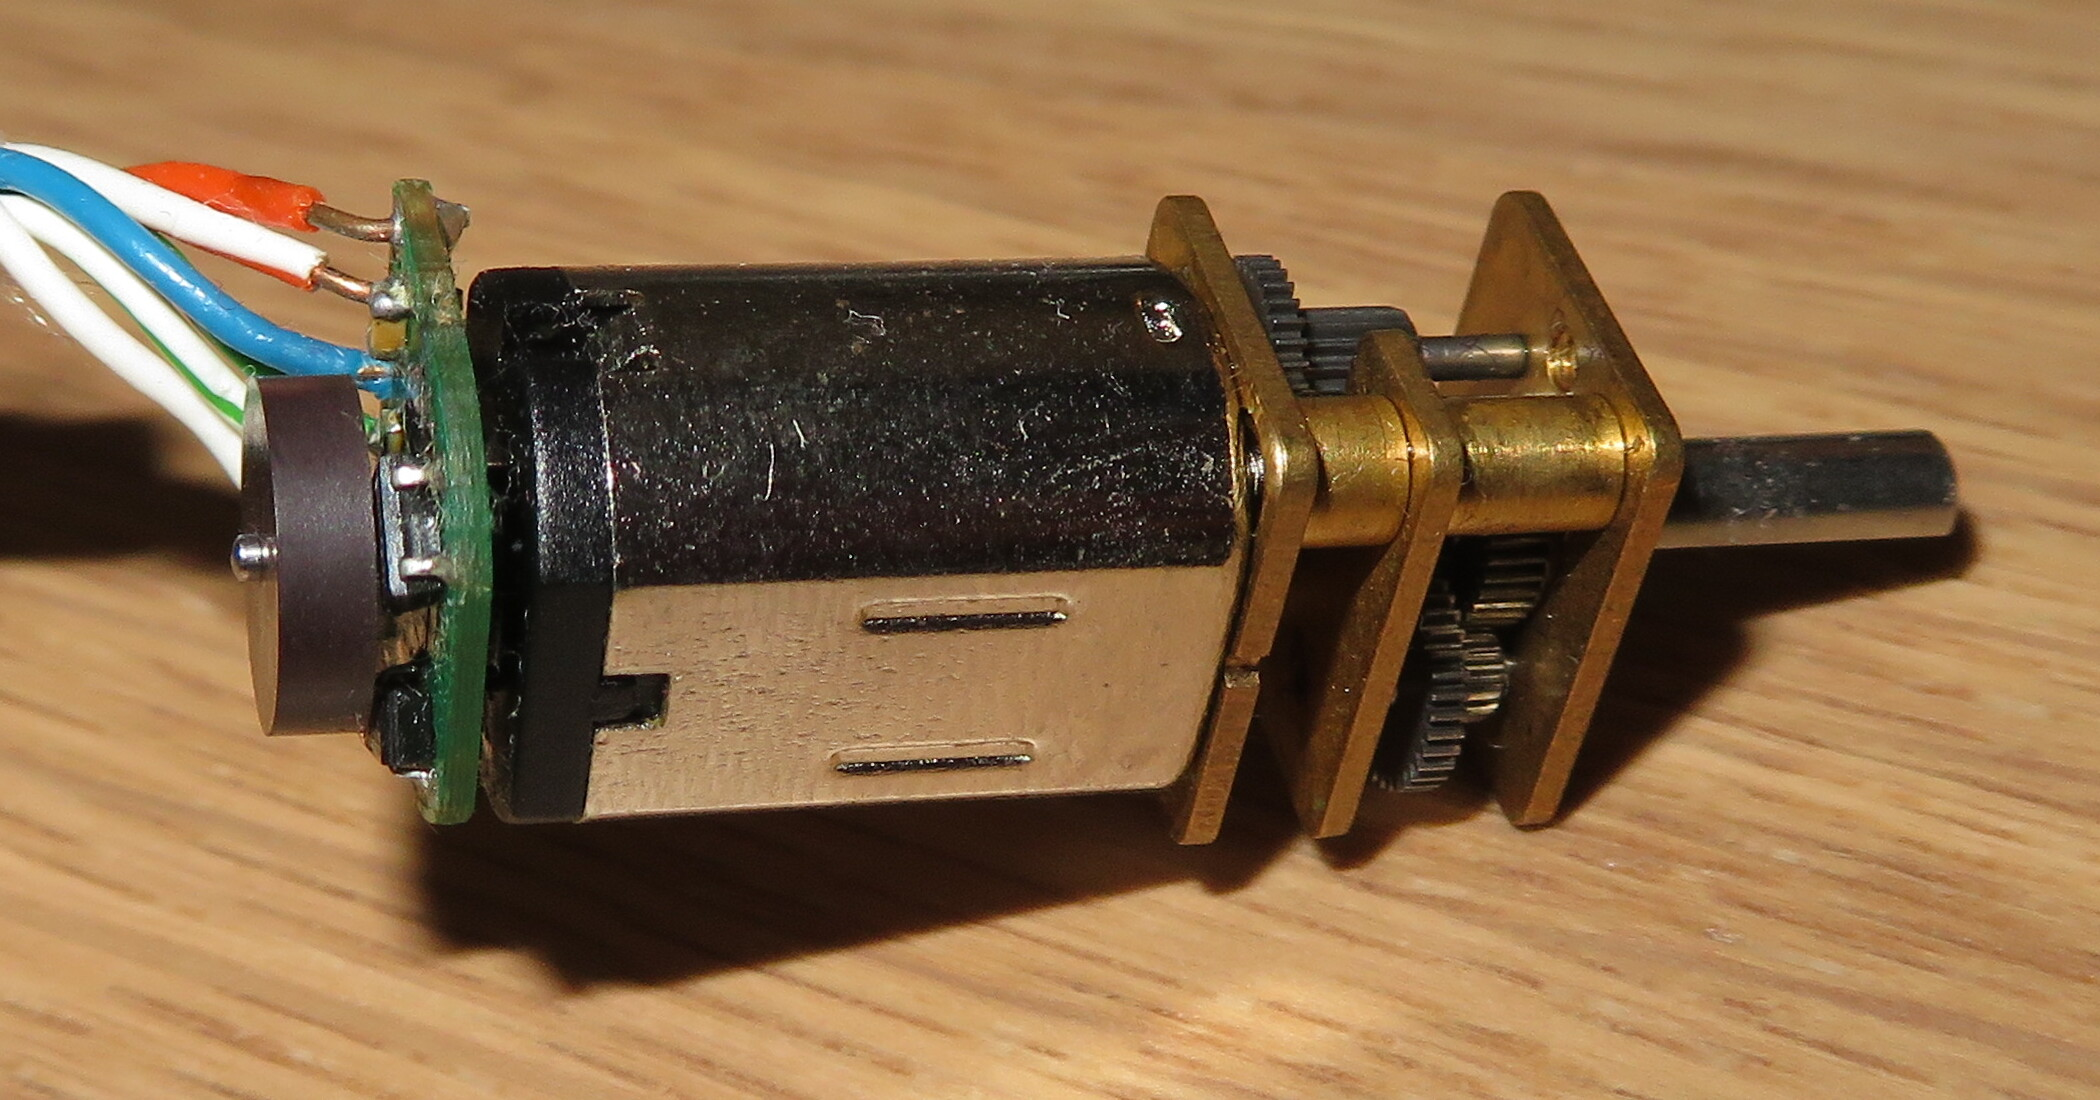
\includegraphics[width=0.8\linewidth]{encoder_motor.JPG}
	\caption{Detail of the DC gearmotor and attached magnetic encoder}
	\label{fig:encoder_motor}
\end{figure}

Incremental quadrature encoders are very commonly used in the industry, mostly due to their simplicity and modest prices, when compared with absolute encoders.
The encoder provides two electrical signals (A and B) which change their values according to the motor angular displacement.
The two electrical signals are said to be in quadrature because they have a phase shift of 90\textdegree{} between them, meaning they will never change state simultaneously.
While rotating, the A and B signals will continuously change their state between 0 and 1, as seen in \autoref{fig:quad-encoder}.
The direction of rotation can be determined by evaluating the relative phase shift between those signals.
If we take signal A as reference and determine that signal B has a +90\textdegree{} phase shift relative to A while rotation clockwise, then a counter-clockwise rotation will generate a B signal with a -90\textdegree{} phase shift relative to A.

\begin{figure}[htp]
	\centering
	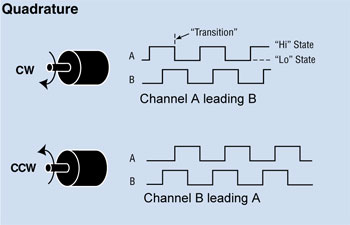
\includegraphics[width=0.8\linewidth]{quad-encoder.jpg}
	\caption{Working principle of an incremental quadrature encoder (Adapted from \cite{technology:quad-encoder})}
	\label{fig:quad-encoder}
\end{figure}

An encoder that is said to have a resolution of 12PPR in quadrature mode means that each quadrature signal (A and B) will generate 3 pulses per revolution.
Therefore, we can catch 6 state changes on each of those signals, providing us a total of 12 pulses per revolution, between the two signals.
A example of such counting method can be seen in \autoref{fig:quad-encoder-2}.

\begin{figure}[htp]
	\centering
	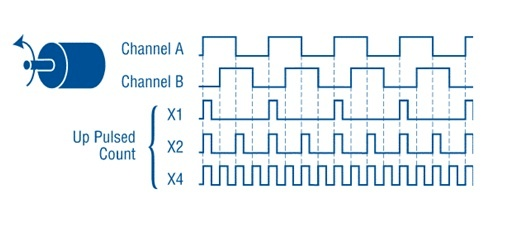
\includegraphics[width=0.8\linewidth]{quad-encoder-2.jpg}
	\caption{Detail of the quadrature count mode (Adapted from \cite{technology:quad-encoder})}
	\label{fig:quad-encoder-2}
\end{figure}

The power supply range allows it to be directly connected to the Raspberry Pi GPIO pins, which only works with 3.3V.
Additionally, the DC motor is rated for a 6V-9V supply.
As the DFR0592 board (see \autoref{subsec:dfr0592}) can provide between 7V and 12V on the motor outputs, depending on the actual power supply used, the entire kit contains components fully compatible between themselves.

Because the DC motor includes a 30:1 reduction gearbox, the resulting encoder precision is multiplied by that ratio, giving the output a virtual encoder resolution of 360 PPR.
For a proof-of-concept system, this is enough precision for position control, providing a maximum error of 1 degree.
This DC motor has a theoretical maximum velocity on the output shaft of 1100 RPM.
This means that encoder pulses will be generated, while at full speed, at a rate of $396000$ pulses per minute, or $6600$ per second.
For velocity control, the maximum amount of pulses generated per second is not too high for the Raspberry Pi, which is perfectly capable of not missing any pulses.

This solution allow us to maintain a low budget for the project and is the main reason we have not chosen to use a standard servo motor paired with a servo drive, although we have considered it.
These two parts would cost more than 400\texteuro, as that was the lowest price we could find on the national market.
Instead, the above mentioned motor and encoder kit summed up to about 30\texteuro, taxes included.

\subsection{DFRobot's DFR0592} \label{subsec:dfr0592}
% Intro
The DFR0592 board from DFRobot is an all-in-one DC motor control board with integrated quadrature encoder interface, PWM generation, an H-bridge for direct motor interface and an integrated micro-controller (an STM32 chip) that takes care of calculating the motor speed in revolutions per minute (RPM).
This board is an add-on HAT for the Raspberry Pi that uses the Inter Integrated Communication (I\textsuperscript{2}C or I2C) protocol to exchange information with the Raspberry Pi.
A preview image of this board can be seen in \autoref{fig:dfr0592-2}.

\begin{figure}[htp]
	\centering
	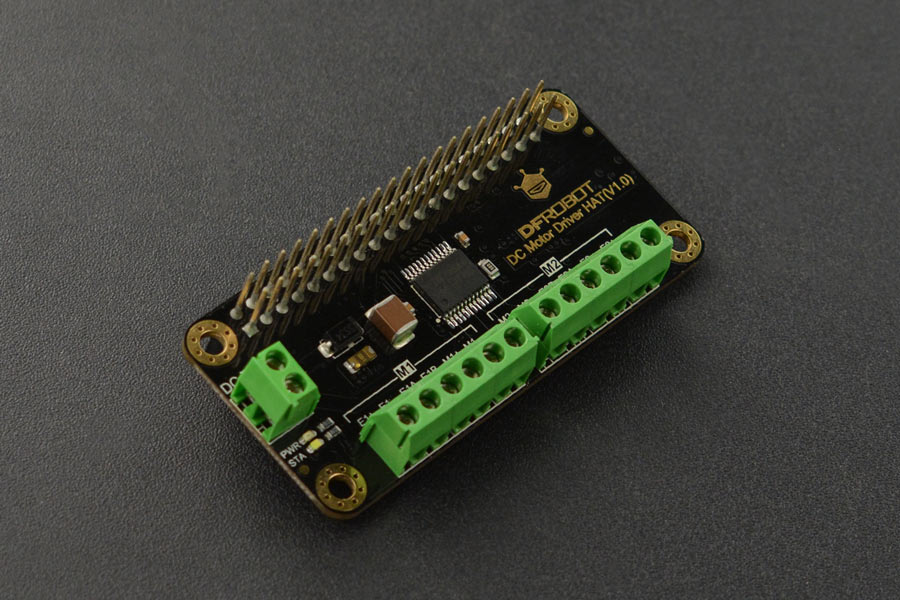
\includegraphics[width=0.8\linewidth]{DFR0592.jpg}
	\caption{DFRobot's DFR0592 board (adapted from \cite{hdw:dfr0592})}
	\label{fig:dfr0592-2}
\end{figure}

% Motor control
This control board takes some configuration values from the Raspberry Pi, such as the motor type (DC or stepper motor), PWM frequency, encoder ratio and others.
For the actual motor control, two values are needed: the direction of rotation (clockwise or counter-clockwise, obviously the motor terminals need to be assigned correctly) and the PWM duty cycle to be used (which is equivalent to saying the percentage of maximum power to apply).

% Conclusions
At first, this board seemed the best fit for the project, but after some preliminary testing, we found that the velocity calculation algorithm was only updating the feedback value every 100ms, which is too great of a period to use for movement control.
It could be acceptable for simple velocity control, but it would also limit the remote operation of the slave device by making it to slow for the desired application.

\subsection{Hilscher's netHAT 52-RTE}
As explained in the previous chapter, our project involves the development of a custom EtherCAT slave device.
For this, we need a specialized hardware interface called an EtherCAT Slave Controller (ESC).
As we have chosen to use a Raspberry Pi as our computing platform, we now require an appropriate ESC HAT board.
We will be using the Hilscher's netHAT 52-RTE \cite{hdw:nethat-52rte} board mostly because FEUP / DEEC had a set of them available for immediate use, so we did not have the necessity to order any for the development of the project.
A preview picture of this board can be seen in \autoref{fig:nethat-52-rte-2}.

\begin{figure}[htp]
	\centering
	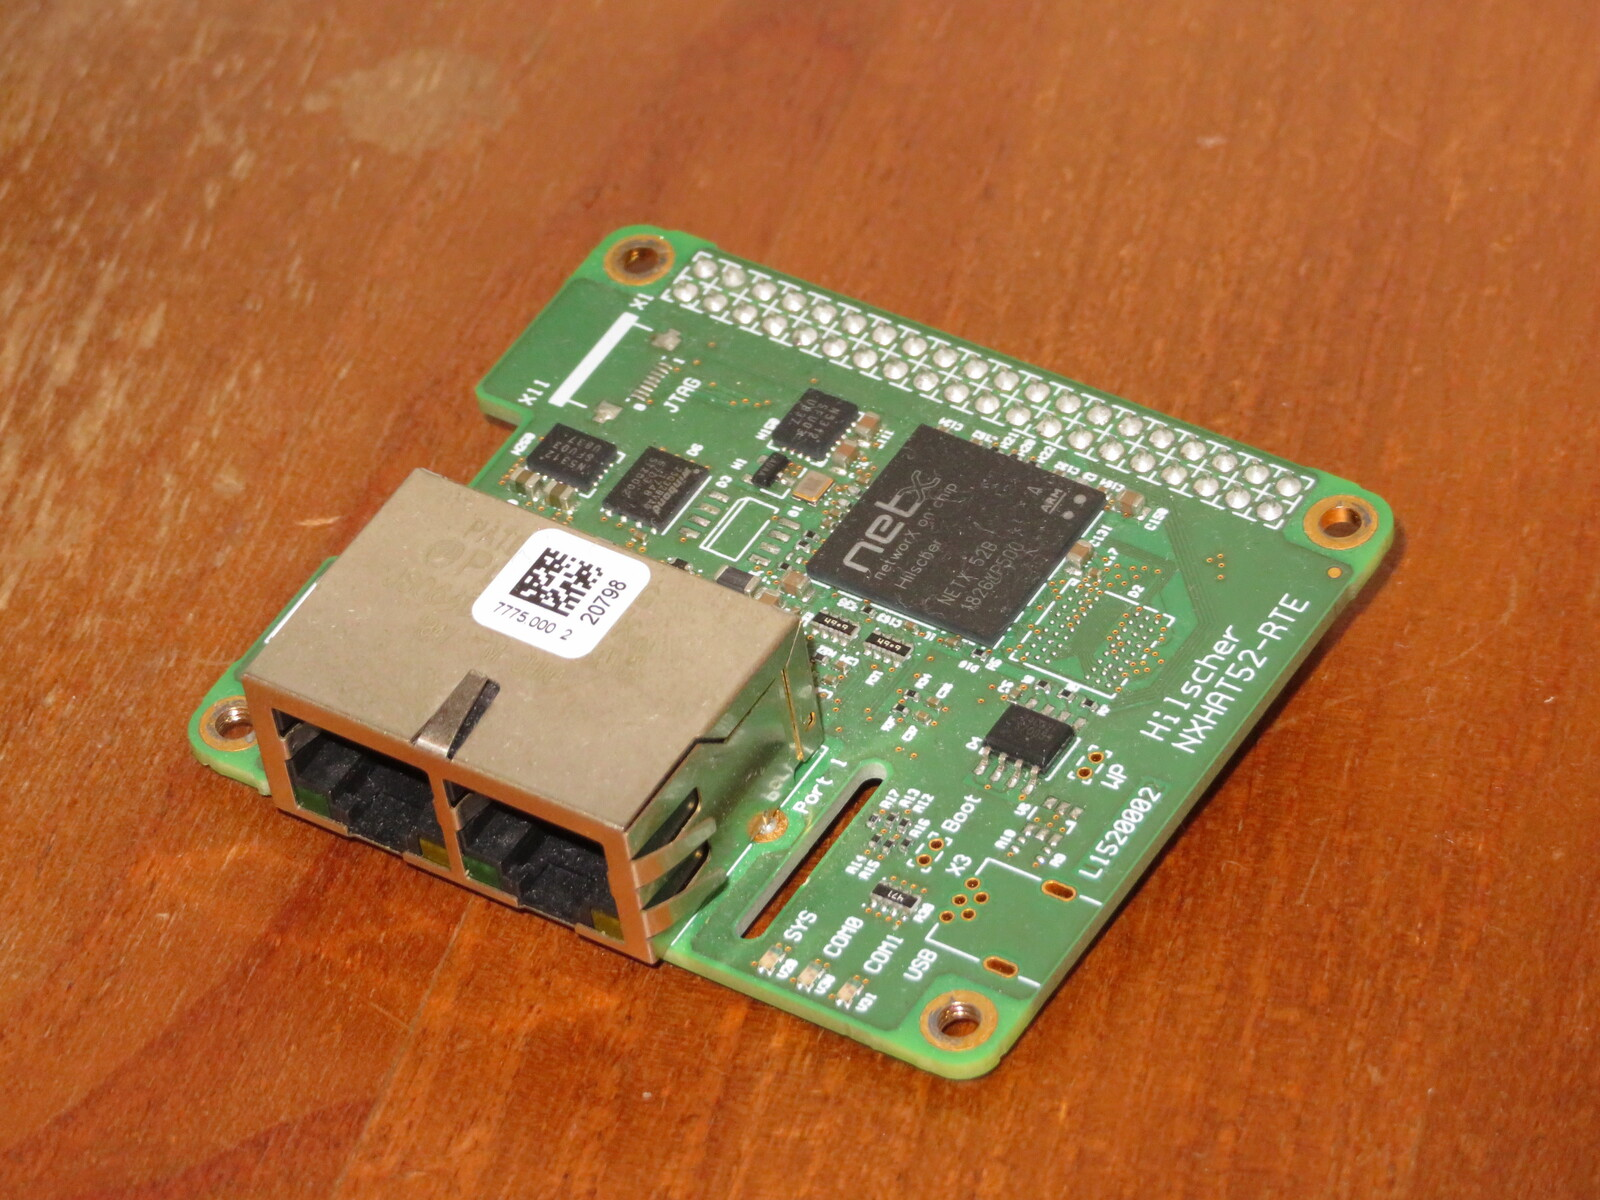
\includegraphics[width=0.8\textwidth]{nethat_52rte.JPG}
	\caption{Hilscher's netHAT 52-RTE board}
	\label{fig:nethat-52-rte-2}
\end{figure}

% HDW specs
The netHAT 52-RTE board has two Ethernet ports so that most of the supported EtherCAT network topologies can be implemented without the need for additional network hardware.
This board uses the Serial Peripheral Interface 0 (SPI0) of the Raspberry Pi for communication and uses a mailbox system to deliver messages to the control program.
The ESC chip allows cyclic synchronisation of 32 bytes of input and 32 bytes of output data.
Considering our project will only require a few bytes for each data type, there is plenty of room to do so.

% SW stuff
This board provides an API library for the C language so developers can program the desired slave device behaviour.
The documentation manuals (\cite{nethat:cifx_api_docs} and \cite{nethat:ethercat_api_docs}) provide useful and insightful information on how this ESC board works and how to use it properly.
These were the main references used during the development of the slave device software, especially during the development of the helper function that interact with the netHAT API library.

\subsection{Screw terminal GPIO interface}
This piece of hardware was necessary in order to connect the above mentioned motor encoder to the Raspberry Pi.
The previously referred stack boards do not provide any external access to the Raspberry Pi's GPIO pins and the Hilscher's netHAT 52-RTE board forces its placement on the top of the stack without providing a pass-through connector.

This specific model has been chosen for its simplicity, reduced cost and ease of use, as connecting the encoder wires is very easy and it provides a stable electrical connection due to the usage of screw terminals.
Unfortunately this model has been discontinued but any generic GPIO expansion board should do the job of exporting the electrical connection needed to interface with the encoder.
